% Options for packages loaded elsewhere
\PassOptionsToPackage{unicode}{hyperref}
\PassOptionsToPackage{hyphens}{url}
\PassOptionsToPackage{dvipsnames,svgnames,x11names}{xcolor}
%
\documentclass[
  letterpaper,
  DIV=11,
  numbers=noendperiod,
  oneside]{scrartcl}

\usepackage{amsmath,amssymb}
\usepackage{iftex}
\ifPDFTeX
  \usepackage[T1]{fontenc}
  \usepackage[utf8]{inputenc}
  \usepackage{textcomp} % provide euro and other symbols
\else % if luatex or xetex
  \usepackage{unicode-math}
  \defaultfontfeatures{Scale=MatchLowercase}
  \defaultfontfeatures[\rmfamily]{Ligatures=TeX,Scale=1}
\fi
\usepackage{lmodern}
\ifPDFTeX\else  
    % xetex/luatex font selection
\fi
% Use upquote if available, for straight quotes in verbatim environments
\IfFileExists{upquote.sty}{\usepackage{upquote}}{}
\IfFileExists{microtype.sty}{% use microtype if available
  \usepackage[]{microtype}
  \UseMicrotypeSet[protrusion]{basicmath} % disable protrusion for tt fonts
}{}
\makeatletter
\@ifundefined{KOMAClassName}{% if non-KOMA class
  \IfFileExists{parskip.sty}{%
    \usepackage{parskip}
  }{% else
    \setlength{\parindent}{0pt}
    \setlength{\parskip}{6pt plus 2pt minus 1pt}}
}{% if KOMA class
  \KOMAoptions{parskip=half}}
\makeatother
\usepackage{xcolor}
\usepackage[left=1in,marginparwidth=2.0666666666667in,textwidth=4.1333333333333in,marginparsep=0.3in]{geometry}
\setlength{\emergencystretch}{3em} % prevent overfull lines
\setcounter{secnumdepth}{-\maxdimen} % remove section numbering
% Make \paragraph and \subparagraph free-standing
\ifx\paragraph\undefined\else
  \let\oldparagraph\paragraph
  \renewcommand{\paragraph}[1]{\oldparagraph{#1}\mbox{}}
\fi
\ifx\subparagraph\undefined\else
  \let\oldsubparagraph\subparagraph
  \renewcommand{\subparagraph}[1]{\oldsubparagraph{#1}\mbox{}}
\fi


\providecommand{\tightlist}{%
  \setlength{\itemsep}{0pt}\setlength{\parskip}{0pt}}\usepackage{longtable,booktabs,array}
\usepackage{calc} % for calculating minipage widths
% Correct order of tables after \paragraph or \subparagraph
\usepackage{etoolbox}
\makeatletter
\patchcmd\longtable{\par}{\if@noskipsec\mbox{}\fi\par}{}{}
\makeatother
% Allow footnotes in longtable head/foot
\IfFileExists{footnotehyper.sty}{\usepackage{footnotehyper}}{\usepackage{footnote}}
\makesavenoteenv{longtable}
\usepackage{graphicx}
\makeatletter
\def\maxwidth{\ifdim\Gin@nat@width>\linewidth\linewidth\else\Gin@nat@width\fi}
\def\maxheight{\ifdim\Gin@nat@height>\textheight\textheight\else\Gin@nat@height\fi}
\makeatother
% Scale images if necessary, so that they will not overflow the page
% margins by default, and it is still possible to overwrite the defaults
% using explicit options in \includegraphics[width, height, ...]{}
\setkeys{Gin}{width=\maxwidth,height=\maxheight,keepaspectratio}
% Set default figure placement to htbp
\makeatletter
\def\fps@figure{htbp}
\makeatother
% definitions for citeproc citations
\NewDocumentCommand\citeproctext{}{}
\NewDocumentCommand\citeproc{mm}{%
  \begingroup\def\citeproctext{#2}\cite{#1}\endgroup}
\makeatletter
 % allow citations to break across lines
 \let\@cite@ofmt\@firstofone
 % avoid brackets around text for \cite:
 \def\@biblabel#1{}
 \def\@cite#1#2{{#1\if@tempswa , #2\fi}}
\makeatother
\newlength{\cslhangindent}
\setlength{\cslhangindent}{1.5em}
\newlength{\csllabelwidth}
\setlength{\csllabelwidth}{3em}
\newenvironment{CSLReferences}[2] % #1 hanging-indent, #2 entry-spacing
 {\begin{list}{}{%
  \setlength{\itemindent}{0pt}
  \setlength{\leftmargin}{0pt}
  \setlength{\parsep}{0pt}
  % turn on hanging indent if param 1 is 1
  \ifodd #1
   \setlength{\leftmargin}{\cslhangindent}
   \setlength{\itemindent}{-1\cslhangindent}
  \fi
  % set entry spacing
  \setlength{\itemsep}{#2\baselineskip}}}
 {\end{list}}
\usepackage{calc}
\newcommand{\CSLBlock}[1]{\hfill\break\parbox[t]{\linewidth}{\strut\ignorespaces#1\strut}}
\newcommand{\CSLLeftMargin}[1]{\parbox[t]{\csllabelwidth}{\strut#1\strut}}
\newcommand{\CSLRightInline}[1]{\parbox[t]{\linewidth - \csllabelwidth}{\strut#1\strut}}
\newcommand{\CSLIndent}[1]{\hspace{\cslhangindent}#1}

\KOMAoption{captions}{tableheading}
\makeatletter
\@ifpackageloaded{caption}{}{\usepackage{caption}}
\AtBeginDocument{%
\ifdefined\contentsname
  \renewcommand*\contentsname{Table of contents}
\else
  \newcommand\contentsname{Table of contents}
\fi
\ifdefined\listfigurename
  \renewcommand*\listfigurename{List of Figures}
\else
  \newcommand\listfigurename{List of Figures}
\fi
\ifdefined\listtablename
  \renewcommand*\listtablename{List of Tables}
\else
  \newcommand\listtablename{List of Tables}
\fi
\ifdefined\figurename
  \renewcommand*\figurename{Figure}
\else
  \newcommand\figurename{Figure}
\fi
\ifdefined\tablename
  \renewcommand*\tablename{Table}
\else
  \newcommand\tablename{Table}
\fi
}
\@ifpackageloaded{float}{}{\usepackage{float}}
\floatstyle{ruled}
\@ifundefined{c@chapter}{\newfloat{codelisting}{h}{lop}}{\newfloat{codelisting}{h}{lop}[chapter]}
\floatname{codelisting}{Listing}
\newcommand*\listoflistings{\listof{codelisting}{List of Listings}}
\usepackage{amsthm}
\theoremstyle{plain}
\newtheorem{theorem}{Question}[section]
\theoremstyle{remark}
\AtBeginDocument{\renewcommand*{\proofname}{Proof}}
\newtheorem*{remark}{Remark}
\newtheorem*{solution}{Solution}
\newtheorem{refremark}{Remark}[section]
\newtheorem{refsolution}{Solution}[section]
\makeatother
\makeatletter
\makeatother
\makeatletter
\@ifpackageloaded{caption}{}{\usepackage{caption}}
\@ifpackageloaded{subcaption}{}{\usepackage{subcaption}}
\makeatother
\makeatletter
\@ifpackageloaded{sidenotes}{}{\usepackage{sidenotes}}
\@ifpackageloaded{marginnote}{}{\usepackage{marginnote}}
\makeatother
\ifLuaTeX
  \usepackage{selnolig}  % disable illegal ligatures
\fi
\usepackage{bookmark}

\IfFileExists{xurl.sty}{\usepackage{xurl}}{} % add URL line breaks if available
\urlstyle{same} % disable monospaced font for URLs
\hypersetup{
  pdftitle={Sphincter analysis},
  pdfauthor={Teddy Groves},
  colorlinks=true,
  linkcolor={blue},
  filecolor={Maroon},
  citecolor={Blue},
  urlcolor={Blue},
  pdfcreator={LaTeX via pandoc}}

\title{Sphincter analysis}
\author{Teddy Groves}
\date{}

\begin{document}
\maketitle

\renewcommand*\contentsname{Table of contents}
{
\hypersetup{linkcolor=}
\setcounter{tocdepth}{3}
\tableofcontents
}
\section{Introduction}\label{introduction}

This project aimed to model brain blood vessel measurements of mice
during a treatment protocol designed to elicit stress responses.

Measurements included:

\begin{itemize}
\tightlist
\item
  Whisker stimulation response (vessel diameter before and after
  stimulation)
\item
  Vessel centre and diameter pulsatility
\item
  Red blood cell flow (i.e.~speed and flux)
\item
  Hypertensive challenge response (Correlation between blood pressure
  and diameter under different pressure conditions)
\end{itemize}

We believed that the mechanisms underlying each kind of measurement were
independent, and moreover each measurement required different data
filtering choices. We therefore conducted a separate analysis for each
measurement type.

Our overall modelling approach broadly followed the recommendations in
Gelman et al. (2020). For each analysis, we first constructed a simple
mathematical model of the data generating process, then iteratively
improved it, taking into account estimated predictive performance in and
out of sample, simplicity, interpretability and computational
feasibility.

We decided to employ a Bayesian modelling approach primarily because of
the availability of non-experimental information, particularly
structural information concerning the data making it important to take
into partially pool information between categories given the relatively
small number of measurements. In a Bayesian context partial pooling can
be achieved using a prior distribution on the random effects.

\section{Overall strategy}\label{overall-strategy}

Although our project involved several statistical analyses, we used a
similar overall strategy in each case. This section describes the
aspects of this strategy that were common to all of our analyses.

\subsection{Features}\label{features}

All of our analyses involved a common data structure, with real-valued
measurements each with multiple categorical features, namely

\begin{itemize}
\tightlist
\item
  age of the measured mouse (adult or young)
\item
  identity of the measured mouse
\item
  stage of the treatment protocol when measured
\item
  measured vessel type (penetrating artery, sphincter, bulb, first order
  capilary, etc)
\end{itemize}

\subsection{Data processing}\label{data-processing}

We ignored data from one mouse (id 310321) that was determined to be an
outlier. 310321 is a mouse where we did not see any whisker response, it
reacted to angiotensin II, but the BP increase was abrupted for a short
while and then re-established. Perhaps due to a clot or a bubble in the
venous catheter. This resulted in a biphasic and slow BP increase.

In all of our analyses we assumed that any missing measurements were
caused by factors that were unrelated to our main target process, or in
other words that the absent measurements were ``missing at random''. We
therefore did not attempt to model the measurement removal process
explicitly.

\subsection{Modelling approach}\label{modelling-approach}

All of our models had a common structure, with generalised linear models
used to describe information from measurements and multi-level prior
distributions used to describe non-experimental information. The
modelling choices open to us concerned the following questions:

\begin{enumerate}
\def\labelenumi{\arabic{enumi}.}
\item
  What generalised linear model to use to model measurements?
\item
  Which interaction effects to estimate?
\item
  What structure to use for the prior model, and in particular how and
  to what extent to pool information between categories?
\item
  What quantitative values to use for our prior model?
\item
  In cases where a phenomenon of interest was assessed using multiple,
  potentially related measurements, whether to model the possible
  relatedness?
\end{enumerate}

In order to answer these questions for each analysis, we started with a
simple but plausible model, then iteratively added and removed
components as described in Gelman et al. (2020). Our general aim was to
achieve a better quantitative and qualitative description of the data
generating process while avoiding computational issues. In particular,
we focused on the estimated out of sample predictive performance as
measured by the estimated leave-one-observation-out log predictive
density (Vehtari, Gelman, and Gabry 2017) and qualitative agreement
between predictive and observed observations in graphical checks.

We address these questions below for each analysis in its corresponding
section, providing model comparisons and illustrative results where
appropriate.

\subsection{Software}\label{software}

The raw data are found in csv files which are available from our
project's github repository at the following urls:

\begin{itemize}
\tightlist
\item
  \url{https://github.com/teddygroves/sphincter/blob/main/data/raw/hyper_challenge.csv}
\item
  \url{https://github.com/teddygroves/sphincter/blob/main/data/raw/data_sphincter_paper.csv}
\end{itemize}

For each analysis, we conducted filtering and reshaping operations using
the standard scientific Python stack and validated the resulting
prepared datasets against custom data models constructed using the
Python libraries pydantic (Pydantic developers 2022) and pandera (Niels
Bantilan 2020). These models can be inspected at this url:
\url{https://github.com/teddygroves/sphincter/blob/main/sphincter/data_preparation.py}.

Statistical computation was carried out using the probabilistic
programming framework Stan (Carpenter et al. 2017) via the interface
cmdstanpy (Stan Development Team 2022).

Analysis and serialisation of posterior samples was carried out using
the Bayesian inference library arviz (Kumar et al. 2019).

Our analysis was orchestrated by the Python package bibat (Groves 2023).

\subsection{Validation of statistical
computation}\label{validation-of-statistical-computation}

We validated our statistical computation using standard Hamiltonian
Monte Carlo diagnostics, including the improved \(\hat{R}\) statistic
(Vehtari et al. 2021) as well as inspection for post-warmup divergent
transitions (Betancourt 2017), problematic EBFI statistics, tree depth
or effective sample size to total sample size ratios. All reported
models had improved \(\hat{R}\) close to 1 and no divergent transitions
or other signs of algorithm failure.

\subsection{Reproducibility}\label{reproducibility}

See the repository readme for instructions on reproducing our analysis:
\url{https://github.com/teddygroves/sphincter/blob/main/README.md}

\section{Main findings}\label{main-findings}

\subsection{Whisker stimulation}\label{whisker-stimulation}

Our analysis of whisker stimulation data indicates that the hypertension
and sphincter ablation treatments are associated with lower whisker
stimulation response, as measured by log diameter change, compared with
the baseline treatment. The effect from whisker stimulation is greater
than from hypertension.

Figure Figure~\ref{fig-whisker-treatment-effects} illustrates this
finding by showing the distribution of posterior samples for treatment
effects relative to baseline from our best whisker stimulation model.

\begin{figure}

\begin{minipage}{\linewidth}

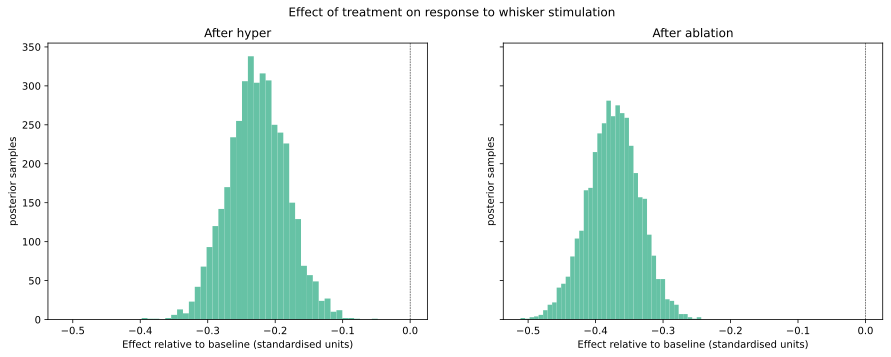
\includegraphics{../plots/whisker-treatment-effects.png}

\end{minipage}%

\caption{\label{fig-whisker-treatment-effects}Marginal posterior
histograms for treatment effects, relative to the baseline treatment.}

\end{figure}%

Our analysis did not indicate any substantial difference between old and
adult mice, or any noticeable vessel type:treatment interaction effects.
This can be seen from figure Figure~\ref{fig-whisker-small-effects},
which shows posterior quantiles for age and vessel type:treatment
interaction effects in our model that included both of these.

\begin{figure}

\begin{minipage}{\linewidth}

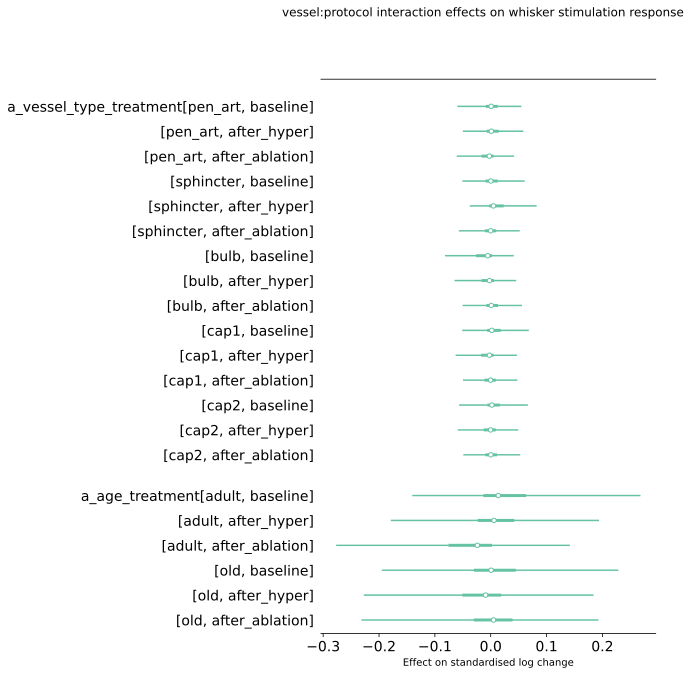
\includegraphics{../plots/whisker-protocol-effects.png}

\end{minipage}%

\caption{\label{fig-whisker-small-effects}Marginal 2.5\%-97.5\%
posterior intervals for protocol effects}

\end{figure}%

We found some difference between vessel type effects: sphincters had the
greatest relative diameter change in response to whisker stimulation,
and bulbs the smallest. Figure
Figure~\ref{fig-whisker-vessel-type-effects} shows these.

\begin{figure}

\begin{minipage}{\linewidth}

\includegraphics{../plots/whisker-vessel-type-effects.png}

\end{minipage}%

\caption{\label{fig-whisker-vessel-type-effects}Marginal 2.5\%-97.5\%
posterior intervals for vessel type effects}

\end{figure}%

\subsection{Pulsatility}\label{pulsatility}

Our analysis of vessel centre and diameter pulsatility yielded the
following conclusions:

\begin{itemize}
\item
  Adult mice have higher vessel diameter pulsatility than old mice,
  whereas old mice have slightly higher centre pulsatility.
\item
  Sphincter ablation correlates with increased diameter pulsatility,
  with no strong interaction effects. On the other hand there is no
  clear effect of sphincter ablation on centre pulsatility.
\end{itemize}

Figure~\ref{fig-pulsatility-age-effects} plots the distribution of age
effect differences (adult minus old) for each measurement type in our
final model. This graph shows that, in this model, the age effect for
adult mice was higher than for old mice in every single posterior
sample: in other words there is a clear trend for older mice to have
lower diameter pulsatility. There is a smaller opposite trend for centre
pulsatility measurements, but it is not clearly separated from zero,
indicating that the direction of the effect is not fully settled.

\begin{figure}

\centering{

\includegraphics{../plots/pulsatility-age-effects.png}

}

\caption{\label{fig-pulsatility-age-effects}Posterior distribution of
age effect differences for each measurement type.}

\end{figure}%

Figure~\ref{fig-pulsatility-treatment-effects} shows the distribution of
posterior draws for sphincter ablation effects compared with the
immediately prior protocol stage (``after hypertension''). The
ablation/diameter parameter is greater than the after
hypertension/diameter parameter in 98\% of posterior samples, whereas
there is no clear effect on centre pulsatility.

\begin{figure}

\centering{

\includegraphics{../plots/pulsatility-treatment-effects.png}

}

\caption{\label{fig-pulsatility-treatment-effects}Posterior distribution
of treatment effect differences for each measurement type.}

\end{figure}%

\subsection{Red blood cell flow}\label{red-blood-cell-flow}

Our main result regarding red blood cell flow is that both RBC speed and
flux tend to be higher in adult mice compared with old mice. Figure
Figure~\ref{fig-flow-age-effects} illustrates this finding by plotting
the relevant marginal posterior histograms.

\begin{figure}

\centering{

\includegraphics{../plots/flow-age-effects.png}

}

\caption{\label{fig-flow-age-effects}Posterior distributions of age
effects on red blood cell speed and flux.}

\end{figure}%

We also quantified treatment effects on red blood cell flow, as shown in
Figure~\ref{fig-flow-treatment-effects}:

\begin{figure}

\centering{

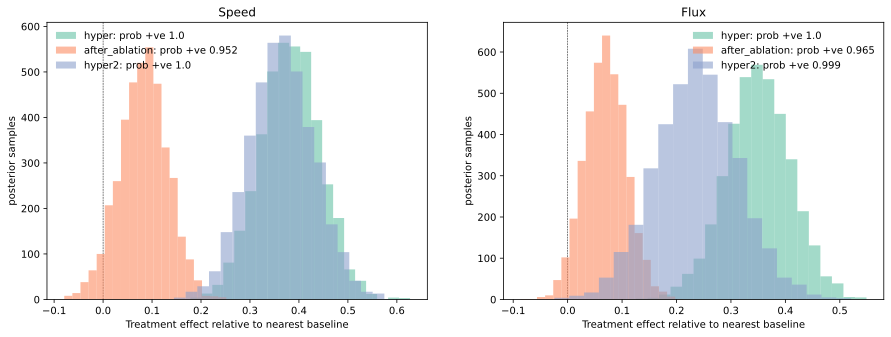
\includegraphics{../plots/flow-treatment-effects.png}

}

\caption{\label{fig-flow-treatment-effects}Posterior distributions of
treatment effects on red blood cell speed and flux. The nearest baseline
for treatment \texttt{hyper} is \texttt{baseline}, and for treatments
\texttt{after\_ablation} and \texttt{hyper2} it is
\texttt{after\_hyper}.}

\end{figure}%

\subsection{Hypertensive challenge}\label{hypertensive-challenge}

Our hypertensive challenge data also showed pronounced age and treatment
differences, as shown in figure Figure~\ref{fig-hypertension-effects}.
Specifically, we found that, for adult mice, blood pressure and vessel
diameter tended to be less correlated, and that the \texttt{hyper2}
treatment tended to increase pressure-diameter correlation compared with
the \texttt{hyper1} treatment.

\begin{figure}

\centering{

\includegraphics{../plots/hypertension-age-and-treatment.png}

}

\caption{\label{fig-hypertension-effects}Posterior distributions of
relative age and treatment effects for hypertensive challenge data.}

\end{figure}%

\subsection{Vessel density}\label{vessel-density}

The vessel density dataset had a somewhat different structure to the
other data, with no treatments, more vessel types, with clear
correlation between measurements corresponding to adjacent vessel types.
We therefore used a different statistical approach, with smoothing
components for parameters of adjacent vessel types. See REF for more
about this model.

Our analysis indicated that the old mice tended to have lower density
than the adult mice for capillaries of order 1 to 3 and higher density
for capillaries of order 9 to 12, and for ascending venules, as shown in
figure Figure~\ref{fig-density-effects}.

\begin{figure}

\centering{

\includegraphics{../plots/density-effects.png}

}

\caption{\label{fig-density-effects}Posterior distributions of
differences in age-dependent parameters by vessel type.}

\end{figure}%

\section{Details of the whisker stimulation
analysis}\label{details-of-the-whisker-stimulation-analysis}

In order to measure how vascular responsiveness changed during our
experimental protocol, the diameters of different vessel types were
recorded before and during whisker stimulation, at baseline,
post-hypertension and post-ablation stages. We aimed to assess
statistical relationships between the known factors and the relative
change in vessel diameter before and after stimulation.

In particular, we were interested in differences between old and adult
mice and in the effect of sphincter ablation.

\subsection{Dependent variable}\label{dependent-variable}

The ratio of the peak compared with the pre-stimulation level for each
mouse at each stage, on natural logarithmic scale, also known as the
`log change', was standardised by subtracting the overall mean and
dividing by the standard deviation, then treated as a single
measurement. This way of the measurements was chosen to facilitate
modelling, as log change is a symmetric and additive measure of relative
change (see Tornqvist, Vartia, and Vartia (1985)).

Note that when the difference between the two values \(v1\) and \(v2\)
is far less than 1, the log change \(\ln{\frac{v2}{v1}}\) is
approximately the same as the more widely used relative difference
measure \(\frac{v2-v1}{v1}\).

\subsection{Statistical Models}\label{statistical-models}

The final model is shown below:

\begin{align}
y_{vtm} &\sim ST(\nu, \hat{y}_{vtm}, \sigma_{t}) \label{eq-whisker-model} \\
\hat{y}_{vtm} &= \mu_a \nonumber \\
  &+ \alpha^{treatment}_{t} \nonumber \\
  &+ \alpha^{vesseltype}_v \nonumber \\
\alpha^{treatment}_t &\sim N(0, \tau^{treatment}) \nonumber \\
\alpha^{vesseltype}_v &\sim N(0, \tau^{vesseltype}) \nonumber \\
\nu &\sim Gamma(2, 0.1) \nonumber \\
\sigma_t &\sim HN(0, 0.5) \nonumber \\
\mu &\sim N(0, 0.7) \nonumber \\
\tau^{treatment} &\sim HN(0, 0.7) \nonumber \\
\tau^{vesseltype} &\sim HN(0, 0.7) \nonumber
\end{align}

In equation \eqref{eq-whisker-model}, the term \(ST\) indicates the
student t distribution, \(N\) indicates the normal distribution,
\(Gamma\) the gamma distribution and \(HN\) the `half-normal'
distribution, i.e.~the normal distribution with support only for
non-negative numbers. Subscripts indicate indexes and superscripts
indicate parameter labels.

This model has independent effects for treatments
(\(\alpha^{treatment}\)), vessel types (\(\alpha^{vessel}\)) and age
(\(\mu\)). The treatment and vessel type effects have hierarchical
priors, reflecting the need to partially pool information between
different treatment and vessel type categories. This structure allows
our model to accommodate the full spectrum between different categories
being highly heterogenous---in this case the corresponding \(\tau\)
parameter will be large---and on the other hand high similarity, leading
to small \(\tau\) parameters. The student t distribution was chosen to
reflect the heavy tails we observed in the data, with the parameter
\(\nu\) controlling the level of heaviness.

The prior standard deviation 0.7 was chosen because it led to what we
judged to be a reasonable allocation of prior probability mass over
possible data realisations. The prior for the student t degrees of
freedom parameter \(\nu\) was set following the recommendation in Juárez
and Steel (2010).

As well as this model, we also present results from a more complex model
that adds vessel type:treatment and age:treatment interaction effects.
The full specification of this ``big'' model is as follows, using the
same notation as equation \eqref{eq-whisker-model}:

\begin{align}
y_{vtm} &\sim ST(\nu, \hat{y}_{vtm}, \sigma_{t}) \label{eq-whisker-model-interaction} \\
\hat{y}_{vtm} &= \mu_a \nonumber \\
  &+ \alpha^{treatment}_{t} \nonumber \\
  &+ \alpha^{vesseltype}_v \nonumber \\
  &+ \alpha^{vesseltype:treatment}_{vt} \nonumber \\
  &+ \alpha^{age:treatment}_{vt} \nonumber \\
\alpha^{treatment}_t &\sim N(0, \tau^{treatment}) \nonumber \\
\alpha^{vessel}_v &\sim N(0, \tau^{vessel}) \nonumber \\
\alpha^{vesseltype:treatment}_{vt} &\sim N(0, \tau^{vesseltype:treatment}) \nonumber \\
\alpha^{age:treatment}_{at} &\sim N(0, \tau^{age:treatment}) \nonumber \\
\nu &\sim Gamma(2, 0.1) \nonumber \\
\sigma &\sim HN(0, 0.5) \nonumber \\
\mu &\sim N(0, 0.7) \nonumber \\
\tau^{treatment} &\sim HN(0, 0.7) \nonumber \\
\tau^{vessel} &\sim HN(0, 0.7) \nonumber \\
\tau^{age:treatment} &\sim HN(0, 0.7) \nonumber \\
\tau^{vesseltype:treatment} &\sim HN(0, 0.7) \nonumber 
\end{align}

\subsection{Results}\label{results}

Figure~\ref{fig-whisker-measurements} shows the observed log change
measurements with colours illustrating the various categorical
information. Note that the measurements have different dispersion
depending on the treatment, indicating a the need for a model with
distributional effects.

\begin{figure}

\begin{minipage}{\linewidth}

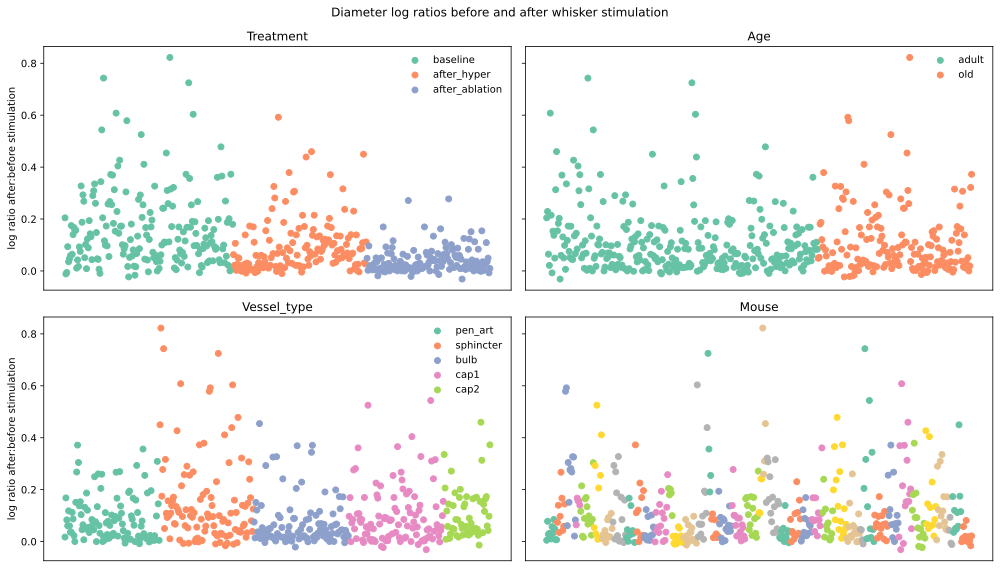
\includegraphics{../plots/whisker-measurements-faceted.png}

\end{minipage}%

\caption{\label{fig-whisker-measurements}Raw measurements}

\end{figure}%

Figure~\ref{fig-whisker-posterior-check} compares the measurements with
our model's posterior predictive distribution. This shows that our model
achieved a reasonable fit to the observed data. There is a pattern in
the model's bad predictions, in that these tend to be for higher
baseline measurements. However, we judged that this pattern was small
enough that for our purposes we could disregard it.

\begin{figure}

\begin{minipage}{\linewidth}

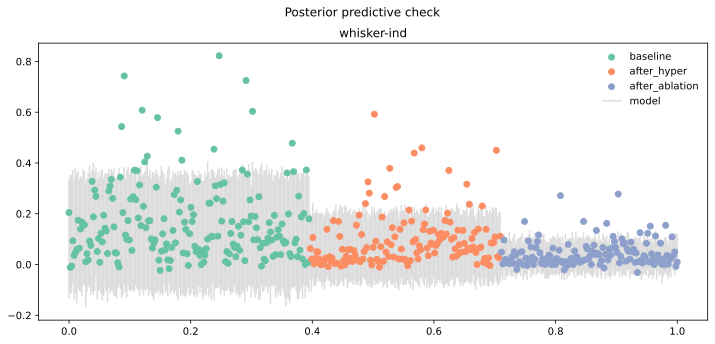
\includegraphics{../plots/whisker-posterior-check-ind.png}

\end{minipage}%

\caption{\label{fig-whisker-posterior-check}Graphical posterior
predictive check}

\end{figure}%

To back up our finding that there were no important interaction effects,
we compared the predictive performance of our final model
\texttt{whisker-ind} with \texttt{whisker-big}, the best-performing
model with more interactions. The results are shown below in figure
Figure~\ref{fig-whisker-loo-compare}:

\begin{figure}

\begin{minipage}{\linewidth}

\includegraphics{../plots/whisker-loo-compare.png}

\end{minipage}%

\caption{\label{fig-whisker-loo-compare}Comparison of estimated
leave-one-oout log predictive density between the final model
\texttt{whisker-ind} and the best performing interaction model
\texttt{whisker-big}.}

\end{figure}%

The two models have similar estimated predictive performance, indicating
that there is no gain from considering interaction effects in this case.

\section{Details of the pulsatility
analysis}\label{details-of-the-pulsatility-analysis}

The pulsatility data consisted of fast measurements of diameter and
center point for the same mice. These measurements were
Fourier-transformed, and the harmonics of the transformed data were
interpreted as representing the pulsatility of the measured quantities.

\subsection{Dependent variable}\label{dependent-variable-1}

We used the first harmonic of each transformed time series as a
dependent variable. It might have been preferable to aggregate all the
available power harmonics, but this would have complicated our
measurement model, and in any case power at the subsequent harmonics was
typically negligible compared with the first.

\subsection{Questions}\label{questions}

As well as the results reported in the main findings section, we were
also interested in these additional questions:

\begin{theorem}[]\protect\hypertarget{thm-qc}{}\label{thm-qc}

How does blood pressure affect diameter and centre pulsatility?

\end{theorem}

\begin{theorem}[]\protect\hypertarget{thm-qd}{}\label{thm-qd}

Do hypertension and sphincter ablation influence diameter and centre
pulsatility differently?

\end{theorem}

\subsection{Description of the
dataset}\label{description-of-the-dataset}

As well as the categorical data described above, our pulsatility
analysis also took into account measurements of each mouse's blood
pressure at the femoral artery.

The final dataset included 514 joint measurements of diameter and centre
pulsatility, calculated as described above. These measurements are shown
in Figure~\ref{fig-pulsatility-dataset}.

\begin{figure}

\begin{minipage}{\linewidth}
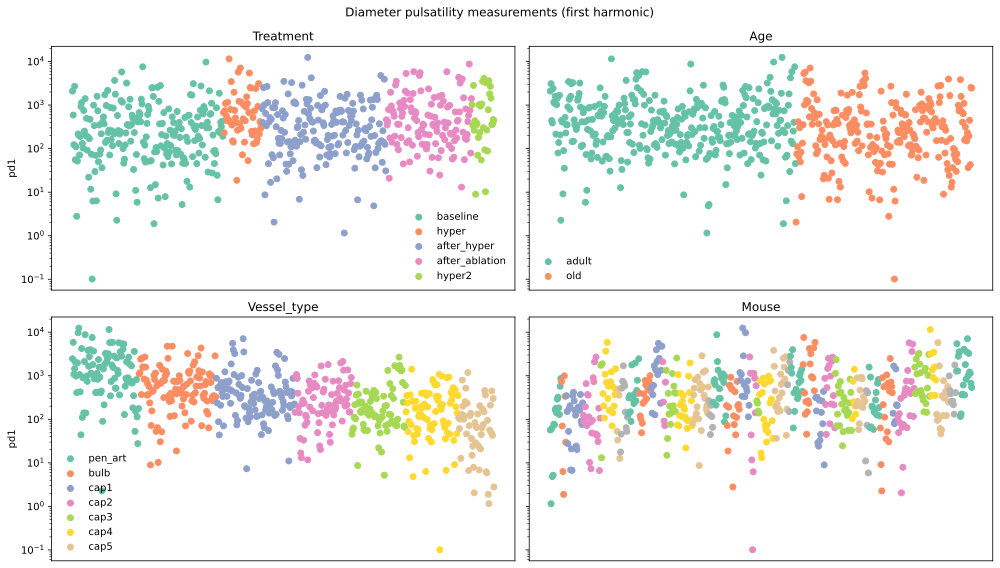
\includegraphics{../plots/pulsatility-diameter-measurements.png}\end{minipage}%
\newline
\begin{minipage}{\linewidth}
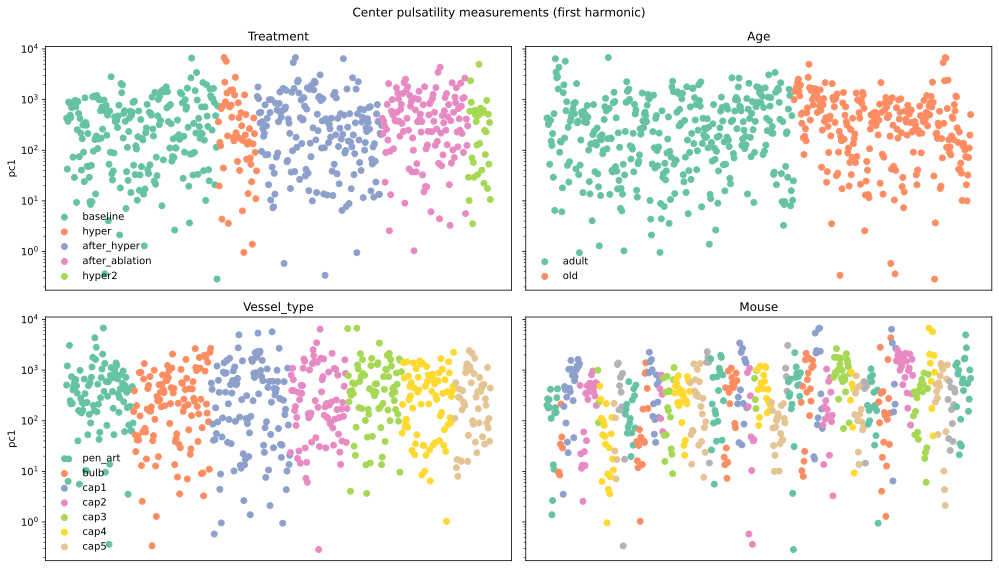
\includegraphics{../plots/pulsatility-center-measurements.png}\end{minipage}%

\caption{\label{fig-pulsatility-dataset}The modelled measurements, shown
in order of the coloured categories.}

\end{figure}%

Figure~\ref{fig-pressure-data} shows the relationship between pressure
and the measurements in our dataset for both age categories. The light
dots show raw measurements and the darker dots show averages within
evenly sized bins.

\begin{figure}

\centering{

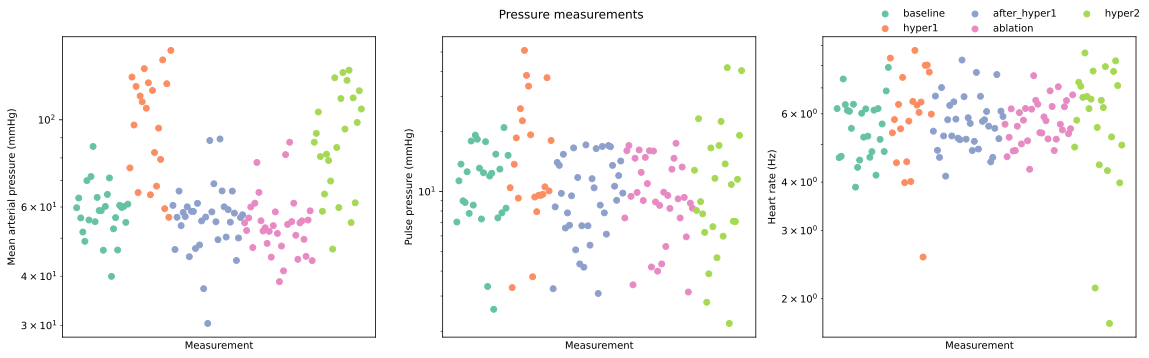
\includegraphics{../plots/pressure-data.png}

}

\caption{\label{fig-pressure-data}Pulsatility measurements plotted
against the corresponding pressure measurements and coloured according
to age. Darker dots indicate averages within evenly sized pressure
bins.}

\end{figure}%

Figure~\ref{fig-diameter-data} shows the relationship between diameter
and the measurements in our dataset for all vessel type categories. The
light dots show raw measurements and the darker dots show averages
within evenly sized bins. There is a clear positive relationship between
measured absolute diameter and diameter pulsatility, and it is
approximately the same for all vessel types.

\begin{figure}

\centering{

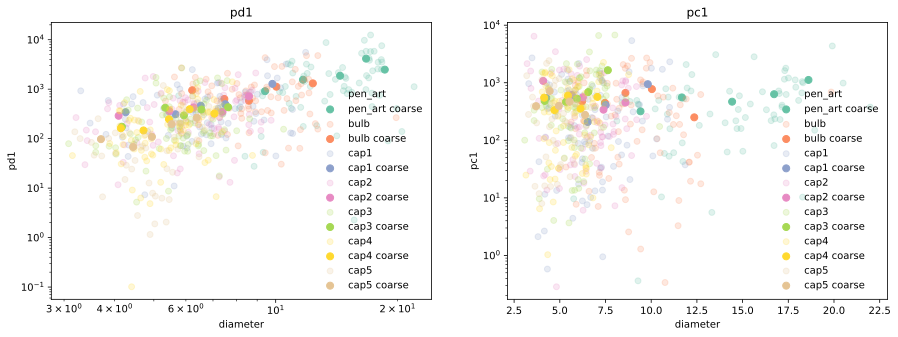
\includegraphics{../plots/pulsatility-diameter-data.png}

}

\caption{\label{fig-diameter-data}Pulsatility measurements plotted
against the corresponding diameter measurements and coloured according
to vessel type. Darker dots indicate averages within evenly sized
pressure bins.}

\end{figure}%

\subsection{Statistical models}\label{statistical-models-1}

We knew from prior studies that the power harmonics should individually
follow exponential distributions {[}REFERENCE FOR THIS{]}. This
consideration motivated the use of exponential generalised linear models
for both the centre and diameter pulsatility measurements. In this
model, given measurement \(y\) and linear predictor \(\eta\) the
measurement probability density is given by this equation:

\begin{align}
  p(y\mid\eta) &= Exponential(y, \lambda) \label{eq:pulsatility-measurement-model}  \\
  &= \lambda e^{-\lambda y}  \nonumber \\
  \ln{\frac{1}{\lambda}} &= \eta \label{eq:link-function}
\end{align}

The log link function \eqref{eq:link-function} was chosen so that linear
changes in the term \(\eta\) induce multiplicative changes in the mean
\(\frac{1}
{\lambda}\) of the measurement distribution, as we believed the effects
we wanted to model would be multiplicative.

We compared four different ways of parameterising \(\eta\) based on the
information available about a given measurement, corresponding to three
hypotheses about the way the data were generated.

The simplest model, which we labelled ``basic'', calculates the linear
predictor \$ \eta\^{}\{basic\}\_\{vtad\}\$ for an observation with
vessel type \(v\), treatment \(t\), age \(a\) and diameter \(d\) as
follows:

\begin{align}
        \label{eq:basic}
    \eta^{basic}_{vtad} &= \mu_{a} \\
      &+ \alpha^{treatment}_{t} \nonumber \\
      &+ \alpha^{vesseltype}_{v} \nonumber \\
      &+ \beta^{diameter} \cdot \ln{d} \nonumber
\end{align}

The basic model provided a plausible baseline against which to compare
the other models.

Next we constructed a more complex model by extending the basic model
with interaction effects, resulting in the following linear predictor:

\begin{align}
        \label{eq:interaction}
    \eta^{interaction}_{vtad} &= \mu_{a} \\
      &+ \alpha^{treatment}_{t} \nonumber  \\
      &+ \alpha^{vesseltype}_{d,vesseltype(n)} \\
      &+ \alpha^{age:treatment}_{at} \nonumber \\
      &+ \alpha^{age:treatment:vesseltype}_{tv} \nonumber \\
    &+ \beta^{diameter}_{d} \cdot \ln{d} \nonumber
\end{align}

Next we constructed a model that adds to the basic model parameters that
aim to capture possible effects corresponding to the blood pressure
measurements. To compensate for collinearity between age and pressure,
our ``pressure'' model does not use the observed pressure as a
predictor, but rather the age-normalised pressure, calculated by
subtracting the mean for each age category from the observed pressure
measurement. The model for the linear predictors \$
\eta\^{}\{pressure\}\_\{vatdp\}\$ with age-normalised pressure
measurement \(p\) is then

\begin{align}
        \label{eq:pressure-model}
    \eta^{pressure}_{vatdp} &= \mu_{a} \\
      &+ \alpha^{treatment}_{t} \nonumber \\
      &+ \alpha^{vesseltype}_{v} \nonumber \\
      &+ \beta^{diameter}_{d} \cdot \ln{d} \nonumber \\
      &+ \beta^{pressure}_{a} \cdot p \nonumber
\end{align}

Finally, we made a model that includes a pressure effect but no
age-specific parameters from the pressure model. This was to test
whether any age effects are due to the collinearity between age and
pressure. The pressure-no-age model's linear predictors
\(\eta^{pressure\ no\ age}_{vatdp}\) are calculated as shown in equation
\eqref{eq:pressure-no-age-model}. Note that, unlike in equation
\eqref{eq:pressure-model}, the \(\mu\) and \(\beta^{pressure}\)
parameters in equation \eqref{eq:pressure-no-age-model} have no age
indexes.

\begin{align}
        \label{eq:pressure-no-age-model}
    \eta^{pressure\ no\ age}_{vatdp} &= \mu \\
      &+ \alpha^{treatment}_{t} \nonumber \\
      &+ \alpha^{vesseltype}_{v} \nonumber  \\
      &+ \beta^{diameter}_{d} \cdot \ln{d} \nonumber \\
      &+ \beta^{pressure} \cdot p \nonumber
\end{align}

In all of our models the \(\alpha\) parameters were given independent,
semi-informative, hierarchical prior distributions to allow for
appropriate information sharing. The \(\beta\) and \(\mu\) parameters
were given independent, semi-informative, non-hierarchical prior
distributions.

\subsection{Results}\label{results-1}

We estimated the leave-one-out log predictive density for each model
using the method described in Vehtari, Gelman, and Gabry (2017) and
implemented in Kumar et al. (2019). The results of the comparison are
shown below in Figure~\ref{fig-pulsatility-elpd-comparison}.

\begin{figure}

\centering{

\includegraphics{../plots/pulsatility-elpd-comparison.png}

}

\caption{\label{fig-pulsatility-elpd-comparison}Comparison of estimated
leave-one-out log predictive density (ELPD) for our pulsatility models.
The main result is that the pressure-no-age and interaction models are
clearly worse than the pressure model, as shown by the separation of the
relevant grey and dotted lines.}

\end{figure}%

We evaluated our models' fit to data using prior and posterior
predictive checking, with the results for the pressure model shown in
Figure~\ref{fig-pressure-ppc}.

\begin{figure}

\begin{minipage}{\linewidth}
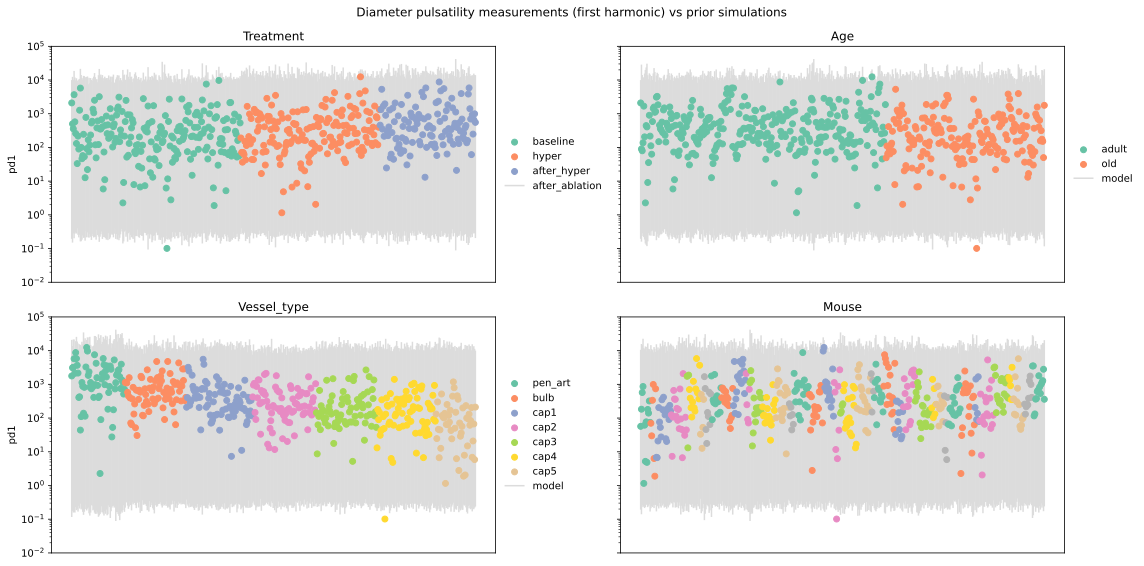
\includegraphics{../plots/pulsatility-prior-check-diameter.png}\end{minipage}%
\newline
\begin{minipage}{\linewidth}
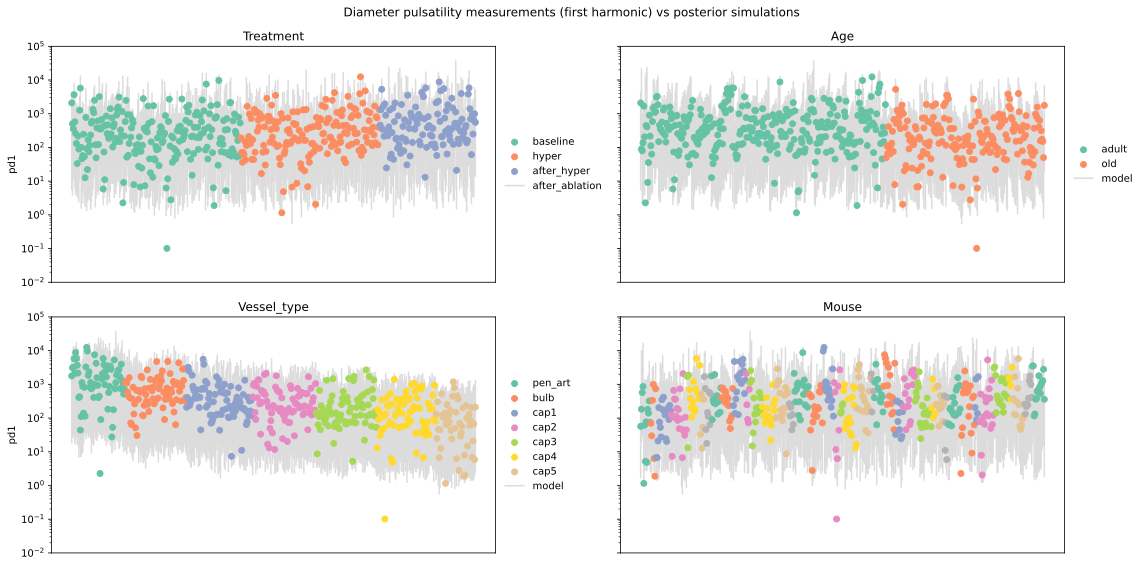
\includegraphics{../plots/pulsatility-posterior-check-diameter.png}\end{minipage}%
\newline
\begin{minipage}{\linewidth}
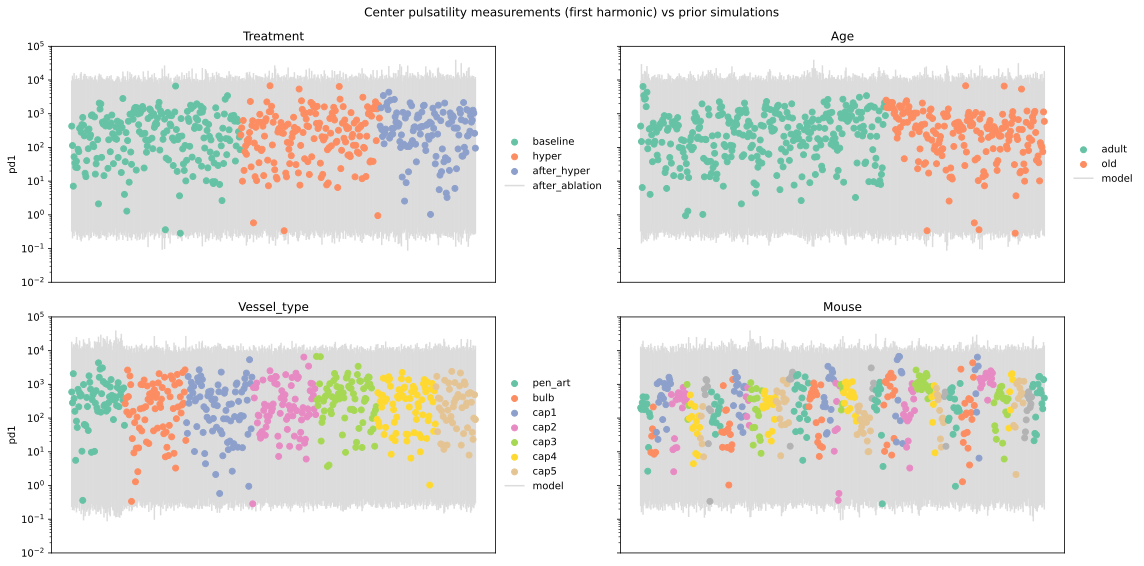
\includegraphics{../plots/pulsatility-prior-check-center.png}\end{minipage}%
\newline
\begin{minipage}{\linewidth}
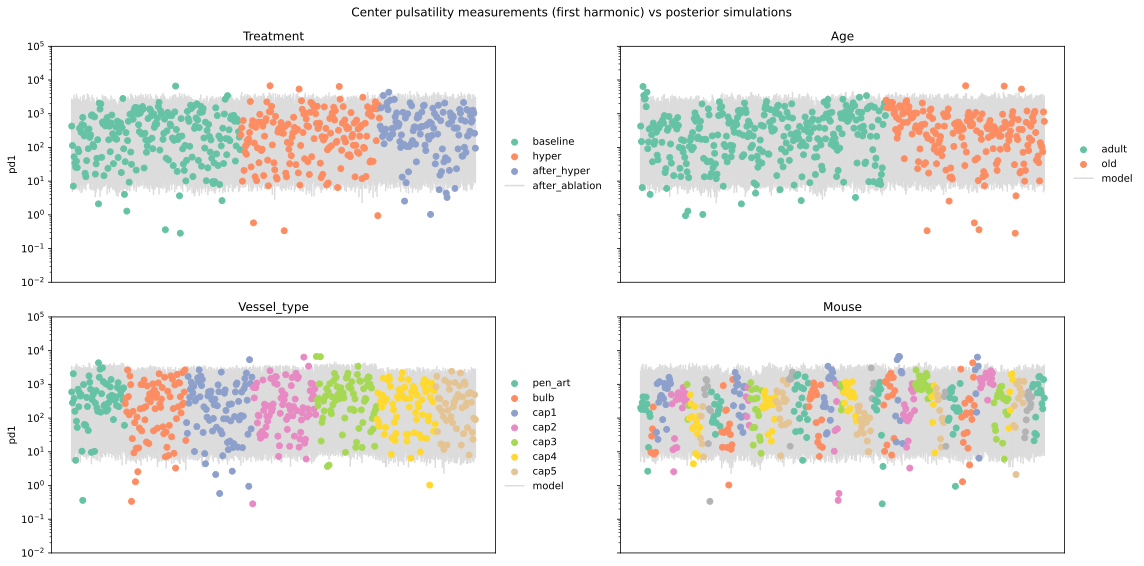
\includegraphics{../plots/pulsatility-posterior-check-center.png}\end{minipage}%

\caption{\label{fig-pressure-ppc}Prior and posterior predictive checks
for the pressure model.}

\end{figure}%

Inspecting of the interaction model output showed that none of the
interaction effect parameters that differed substantially from zero, as
can be seen in Figure~\ref{fig-pulsatility-interaction-effects}.

\begin{figure}

\centering{

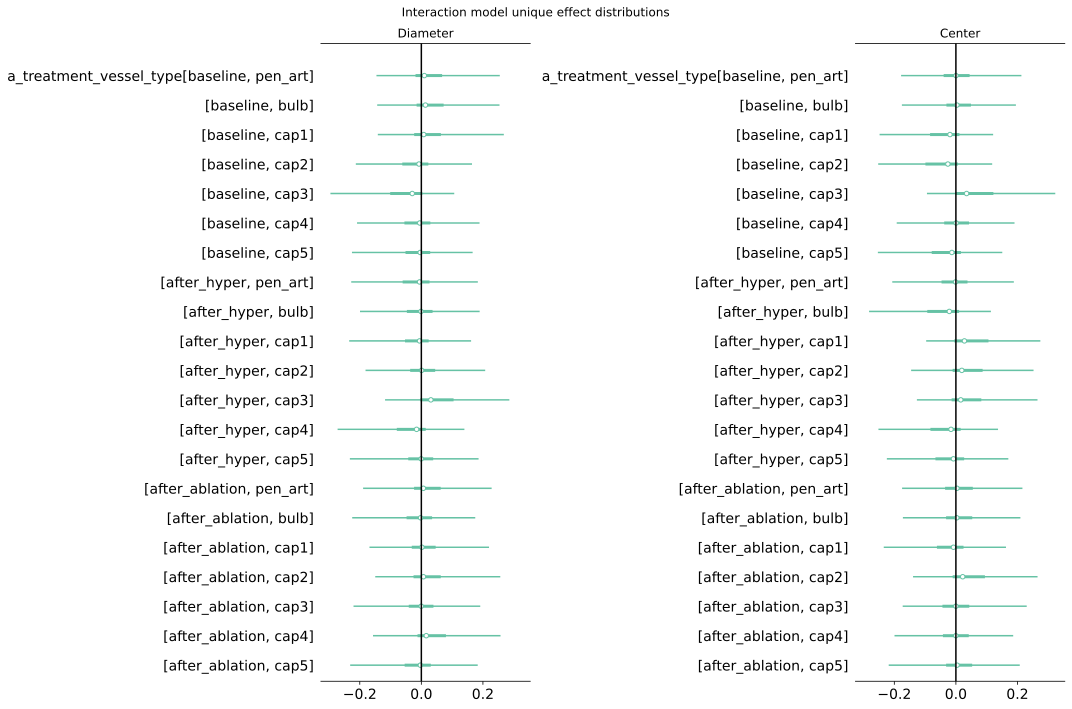
\includegraphics{../plots/pulsatility-interaction-effects.png}

}

\caption{\label{fig-pulsatility-interaction-effects}Marginal posterior
quantiles for the unique effects in the interaction model.}

\end{figure}%

From this result, together with the worse estimated out of sample
predictive performance as shown in
Figure~\ref{fig-pulsatility-elpd-comparison}, we concluded that there
were no important interaction effects, so that we could essentially
discard the interaction model.

Figure~\ref{fig-pulsatility-effects} shows the marginal posterior
distributions for other effect parameters in all three models. Note that
the parameters \texttt{b\_diameter} are strongly positive for diameter
pulsatility in all models and also mostly positive for centre
pulsatility. There is also a strong trend for diameter pulsatility to
decrease with the order of the vessel and no particular vessel type
trend for centre pulsatility.

\begin{figure}

\centering{

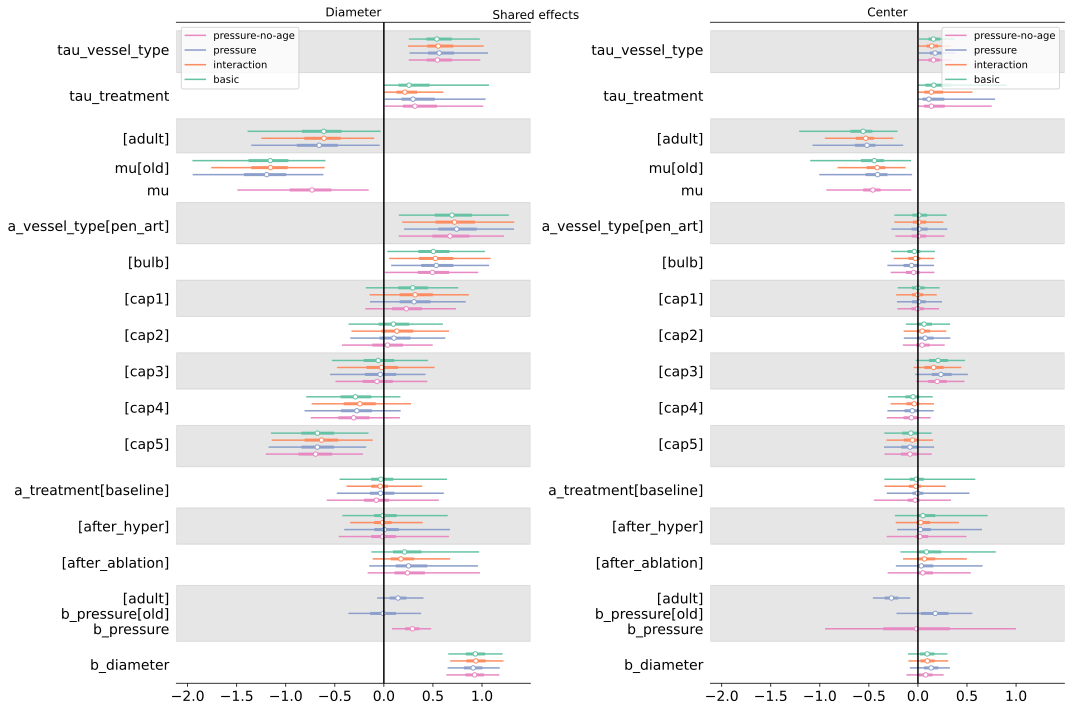
\includegraphics{../plots/pulsatility-effects.png}

}

\caption{\label{fig-pulsatility-effects}Marginal posterior quantiles for
shared model effects.}

\end{figure}%

\subsection{Answers to specific
questions}\label{answers-to-specific-questions}

The poorer estimated out of sample predictive performance of the
pressure-no-age model compared with the other models, as shown in
Figure~\ref{fig-pulsatility-elpd-comparison}, indicates that our
pressure measurements did not fully explain the observed difference
between adult and old mice. It is nonetheless possible that different
pressure explains the difference between old and adult mice, but that
the pressure measurements did not reflect the true pressure at the
measured vessels. This is plausible since the pressure measurements were
taken at a different location.

Figure~\ref{fig-pulsatility-pressure-effects} shows the difference in
\(\beta^{pressure}\) parameters for old and adult mice in the pressure
model in order to answer Question~\ref{thm-qc}. This shows a weak
tendency of the pressure effect on diameter pulsatility to be more
positive for adult mice than for old mice, and a strong opposite
tendency for centre pulsatility. Taking the absolute values into
account, the analysis suggests that greater measured pressure is not
strongly related to diameter pulsatility and correlates with reduced
centre pulsatility for adult mice but not for old mice.

\begin{figure}

\centering{

\includegraphics{../plots/pulsatility-pressure-effects.png}

}

\caption{\label{fig-pulsatility-pressure-effects}Posterior distribution
of pressure effect differences for each measurement type.}

\end{figure}%

To illustrate the effect of treatments, and specifically sphincter
ablation relative to hypertension (i.e.~to answer Question~\ref{thm-qd})
Figure~\ref{fig-pulsatility-treatment-effects} shows the difference
between the effect for each treatment and the baseline treatment effect.
There is a clear effect of ablation to increase diameter pulsatility and
no clear effects of hypertension on diameter pulsatility or of either
treatment on centre pulsatility.

\begin{figure}

\centering{

\includegraphics{../plots/pulsatility-treatment-effects.png}

}

\caption{\label{fig-pulsatility-treatment-effects}Posterior distribution
of treatment effect differences for each measurement type.}

\end{figure}%

To get an idea about how the effect of sphincter ablation on diameter
pulsatility compares quantitatively with the effect of hypertension, we
fit the basic model to the full dataset, without excluding measurements
from either hypertension treatment.
Figure~\ref{fig-pulsatility-treatment-effects-full} shows the main
result from fitting this model: ablation and hypertension had similarly
positive effects on diameter pulsatility. Interestingly there is no
clear effect from the second hypertension treatment.

\begin{figure}

\centering{

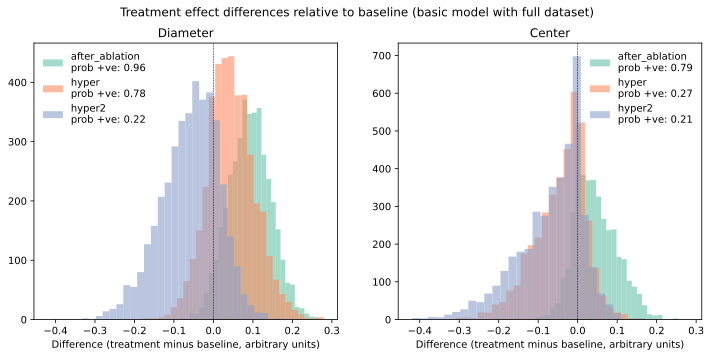
\includegraphics{../plots/pulsatility-treatment-effects-full.png}

}

\caption{\label{fig-pulsatility-treatment-effects-full}Treatment effect
distributions relative to baseline in the basic model when fit to the
full dataset including all treatments.}

\end{figure}%

\section{Details of the red blood cell flow
analysis}\label{details-of-the-red-blood-cell-flow-analysis}

Our measurements included flow data recording the measured speed and
flux of red blood cells through some vessels. This data is interesting
because it allows for inference of the local blood pressure, which
determines the speed.

We were interested in whether the speed and flux tended to be different
between old and adult mice for a given vessel type and treatment, as
this would indicate that the pressure would likely be similar as well.

\subsection{Data processing}\label{data-processing-1}

There is a significant missing data issue in this case: both speed and
flux measurements were available for only 271 out of 1525 raw
measurements. We therefore conducted separate analyses for speed and
flux even though we suspected that these two quantities are related.

\subsection{Dependent variable}\label{dependent-variable-2}

We modelled speed and flux measurements on natural logarithmic scale as
we expected multiplicative effects and this transformation ensures
support on the whole real number line, simplifying modelling.

The resulting measurements are shown in figure
Figure~\ref{fig-flow-data}.

\begin{figure}

\centering{

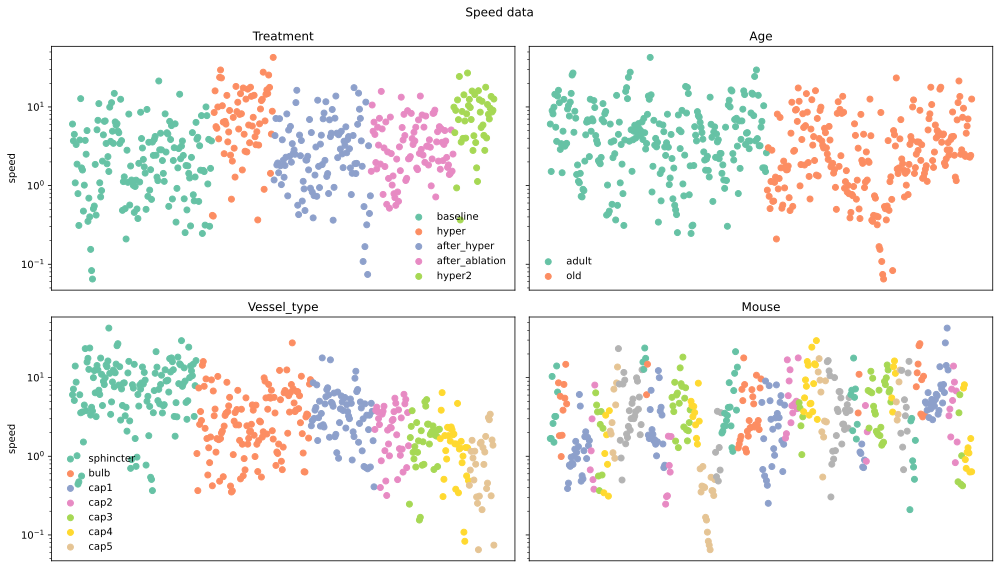
\includegraphics{../plots/flow-speed-measurements.png}

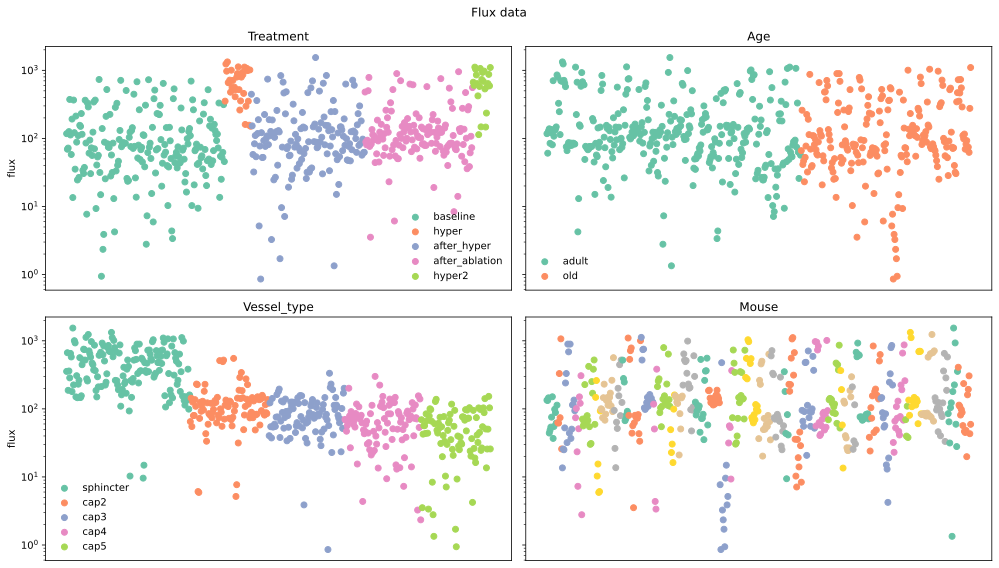
\includegraphics{../plots/flow-flux-measurements.png}

}

\caption{\label{fig-flow-data}Red blood cell speed and flux data}

\end{figure}%

From a glance at these graphs it is clear that there were treatment
effects on both measurement types, particularly from the hypertension
treatments, that there are treatment-related distributional effects, and
that both speed and flux reduce as vessel order increases.

\subsubsection{Statistical models}\label{statistical-models-2}

As in the whisker case we investigated the results of fitting models
with and without interaction effects. Again we found no large or fully
resolved interactions and therefore used the smaller model for further
analysis.

Our final model had this specification:

\begin{align}
\ln(y_{vtm}) &\sim N(\hat{y}_{vtm}, \sigma_t) \label{eq-flow-model} \\
\hat{y}_{vtm} &= \mu_a \nonumber \\
  &+ \alpha^{treatment}_{t} \nonumber \\
  &+ \alpha^{vesseltype}_{v} \nonumber \\
\alpha^{treatment}_t &\sim N(0, \tau^{treatment}) \nonumber \\
\alpha^{vesseltype}_v &\sim N(0, \tau^{vesseltype}) \nonumber \\
\sigma_t &\sim HN(0, 0.5) \nonumber \\
\mu &\sim N(0, 0.5) \nonumber \\
\tau^{treatment} &\sim HN(0, 0.5) \nonumber \\
\tau^{vesseltype} &\sim HN(0, 0.5) \nonumber
\end{align}

We chose the prior standard deviation 0.5 after prior predictive
checking to ensure reasonably tight coverage of the observed data.

For investigation of interaction effects we fit another model that
extended our final model with a vessel type:treatment interaction effect
as follows:

\begin{align}
\hat{y}_{vtm} &= \mu_a \nonumber \\
  &+ \alpha^{treatment}_{t} \nonumber \\
  &+ \alpha^{vesseltype}_{v} \nonumber \\
  &+ \alpha^{vesseltype:treatment}_{vt} \nonumber \\
\alpha^{vesseltype:treatment}_v &\sim N(0, \tau^{vesseltype:treatment}) \nonumber \\
\tau^{vesseltype:treatment} &\sim HN(0, 0.5) \nonumber
\end{align}

\subsection{Results}\label{results-2}

Our statistical model successfully captured all of these trends, as can
be seen from figure Figure~\ref{fig-flow-ppc}

\begin{figure}

\centering{

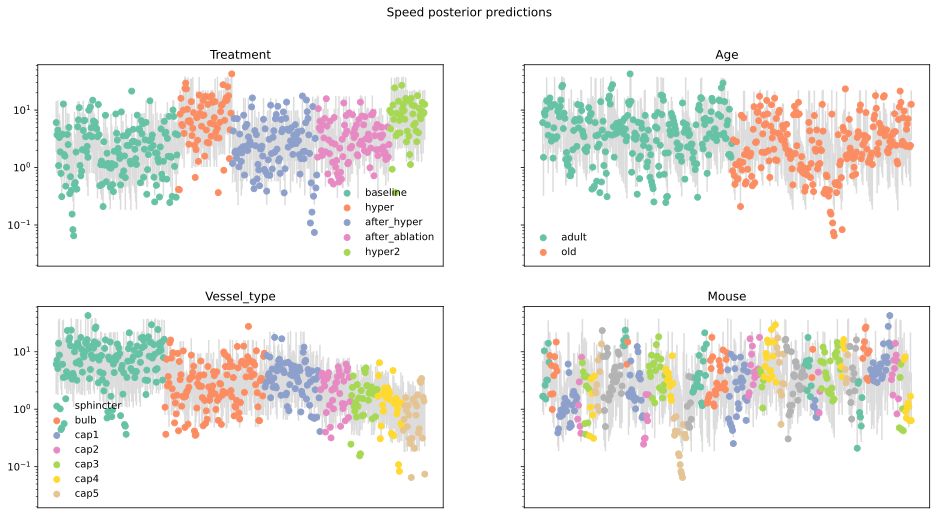
\includegraphics{../plots/flow-basic-speed-posterior-predictive.png}

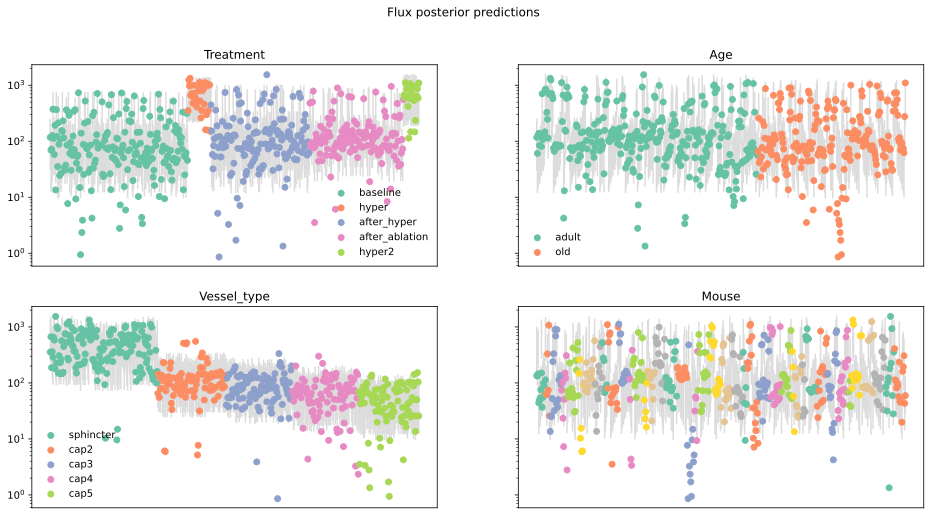
\includegraphics{../plots/flow-basic-flux-posterior-predictive.png}

}

\caption{\label{fig-flow-ppc}Posterior predictive checks for flow
models}

\end{figure}%

\subsubsection{Shared parameters}\label{shared-parameters}

Figure~\ref{fig-flow-shared} summarises the marginal posterior
distributions for parameters that appear in both our final flux and
speed models. There is quite a lot of agreement, unsurprisingly given
that red blood cell speed and flux are closely related. We conclude from
this plot that, given sufficient data, a joint model including both
measurement types would be a good topic for future analysis.

It is also interesting to note the main area where our flux and speed
models disagree, namely the effect corresponding the vessel type
sphincter. According to our model, the sphincter tends to have the
lowest RBC speed of all vessels but the highest flux.

\begin{figure}

\centering{

\includegraphics{../plots/flow-shared-parameters.png}

}

\caption{\label{fig-flow-shared}Posterior distributions of parameters
that appear in both our flow and speed models.}

\end{figure}%

\subsubsection{Interactions}\label{interactions}

To test for important interaction effects we fit a model with vessel
type:treatment interaction parameters. This model achieved marginally
worse loo elpd scores as shown in figure Figure~\ref{fig-flow-loo}.

\begin{figure}

\centering{

\includegraphics{../plots/flow-loo.png}

}

\caption{\label{fig-flow-loo}Out of sample predictive performance
comparison for red blood cell flow models.}

\end{figure}%

For completeness the interaction effects are shown in figure
Figure~\ref{fig-flow-interaction}. No effects are clearly separated from
zero. The sphincter/ablation effect on RBC speed is notably different
from the others. We fit several models with sparsity-inducing priors
including the regularised horseshoe Piironen and Vehtari (2017) to see
if it was possible to resolve this effect, but were unsuccessful. From
this we conclude that any real effect is too small to be easily detected
in our dataset.

\begin{figure}

\centering{

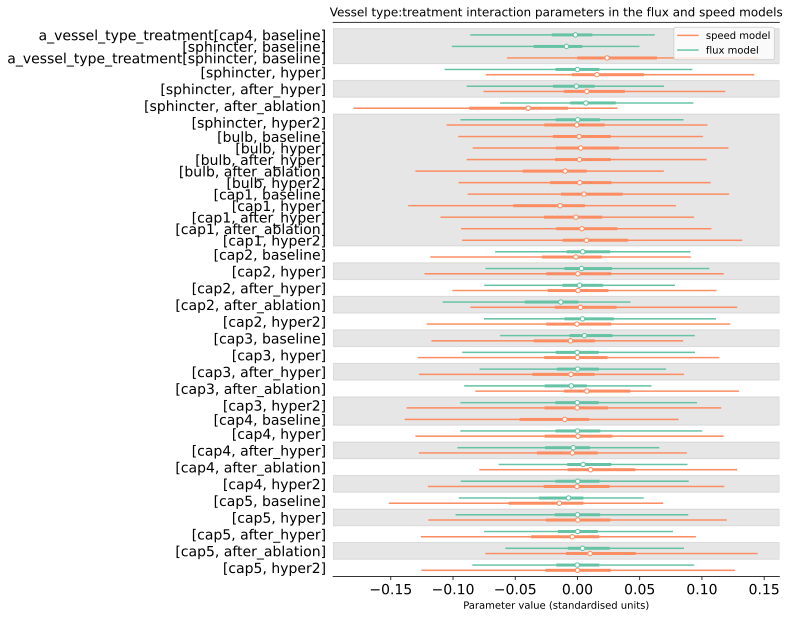
\includegraphics{../plots/flow-interaction-parameters.png}

}

\caption{\label{fig-flow-interaction}Interaction effects on red blood
cell flow.}

\end{figure}%

\section{Hypertensive challenge}\label{hypertensive-challenge-1}

\subsection{Dependent variable}\label{dependent-variable-3}

The raw data on hypertension challenge were correlation coefficients
relating blood pressure and vessel diameter, which are constrained to
lie on the \([-1,
1]\) interval. For easier modelling we transformed these by applying an
inverse hyperbolic tangent function for use in modelling. The dependent
variables then had support on the entire real number line.

The resulting dataset is shown in figure
Figure~\ref{fig-hypertension-data}. The transformed correlation
coefficients do not appear extremely dispersed, indicating that standard
modelling techniques ought to be able to describe them.

\begin{figure}

\centering{

\captionsetup{labelsep=none}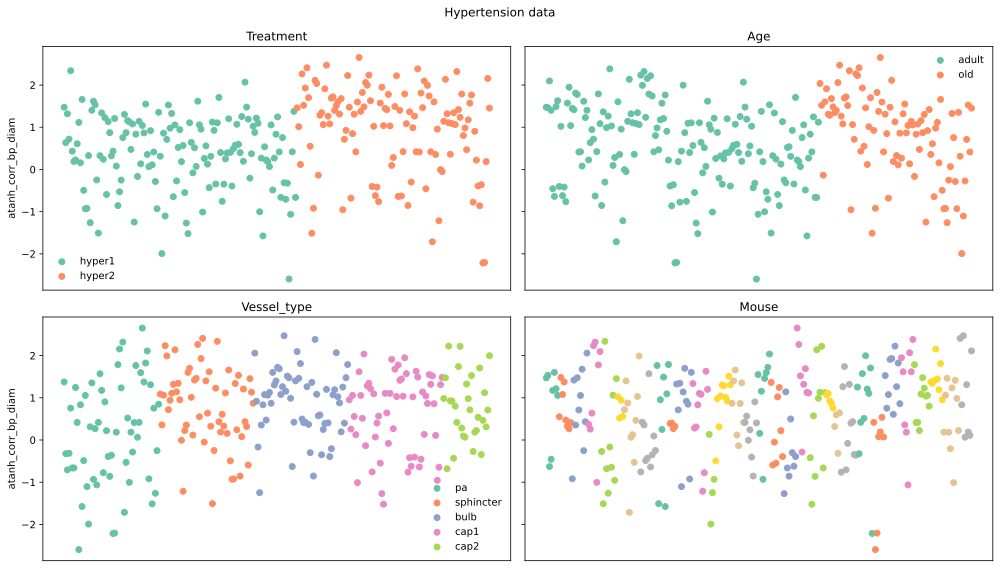
\includegraphics{../plots/hypertension-data.png}

}

\caption{\label{fig-hypertension-data}}

\end{figure}%

\subsubsection{Statistical model}\label{statistical-model}

Our final statistical model had the following form.

\begin{align}
\ln(y_{vtm}) &\sim N(\hat{y}_{vtm}, \sigma_v) \label{eq-hypertension-model} \\
\hat{y}_{vtm} &= \mu_a \nonumber \\
  &+ \alpha^{treatment}_{t} \nonumber \\
  &+ \alpha^{vesseltype}_{v} \nonumber \\
\alpha^{treatment}_t &\sim N(0, 0.5) \nonumber \\
\alpha^{vesseltype}_v &\sim N(0, \tau^{vesseltype}) \nonumber \\
\sigma_v &\sim HN(0, 0.5) \nonumber \\
\mu &\sim N(0, 0.5) \nonumber \\
\tau^{vesseltype} &\sim HN(0, 0.5) \nonumber
\end{align}

This model is different from the others in that we did not partially
pool the treatment effects, since there were only two of these in this
case. We also allowed the measurement error parameters \(\sigma\) to
vary according to vessel type, since this improved model fit and
predictive performance.

As in the other analyses, for investigation of interaction effects we
fit another model that extended our final model with a vessel
type:treatment interaction effect as follows:

\begin{align}
\hat{y}_{vtm} &= \mu_a \nonumber \\
  &+ \alpha^{treatment}_{t} \nonumber \\
  &+ \alpha^{vesseltype}_{v} \nonumber \\
  &+ \alpha^{vesseltype:treatment}_{vt} \nonumber \\
\alpha^{vesseltype:treatment}_v &\sim N(0, \tau^{vesseltype:treatment}) \nonumber \\
\tau^{vesseltype:treatment} &\sim HN(0, 0.5) \nonumber
\end{align}

\subsection{Results}\label{results-3}

Figure~\ref{fig-hypertension-loo} shows that, as in the other cases,
including interaction effects did not improve estimated predictive
performance.

\begin{figure}

\centering{

\includegraphics{../plots/hypertension-loo.png}

}

\caption{\label{fig-hypertension-loo}Comparison of out-of-sample
predictive performance of our hypertension models, as measured by
estimated leave-one-out expected log predictive density. The two models
have similar estimated performance, but the \texttt{hypertension-big}
model is clearly worse.}

\end{figure}%

Figure~\ref{fig-hypertension-parameters} shows the marginal
distributions for the non-hierarchical parameters in our final model.

\begin{figure}

\centering{

\includegraphics{../plots/hypertension-parameters.png}

}

\caption{\label{fig-hypertension-parameters}1\%-99\% posterior intervals
for parameters in our final hypertension model.}

\end{figure}%

Figure~\ref{fig-hypertension-predictions} shows graphical prior and
posterior predictive checks for our final hypertension model. The fit is
fairly good, with no obvious systematic pattern in the errors, though
slightly more observations lie outside the plotted intervals than might
be expected.

\begin{figure}

\centering{

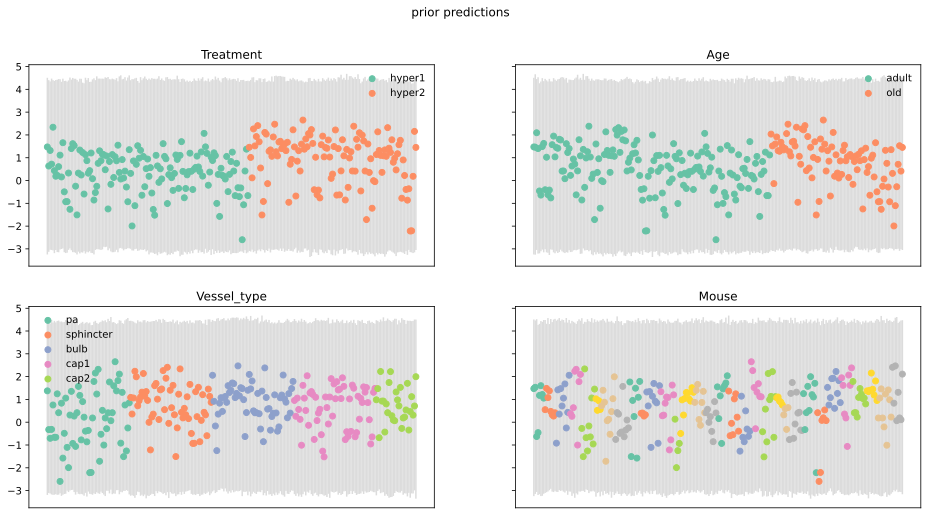
\includegraphics{../plots/hypertension-prior-predictive.png}

}

\caption{\label{fig-hypertension-predictions}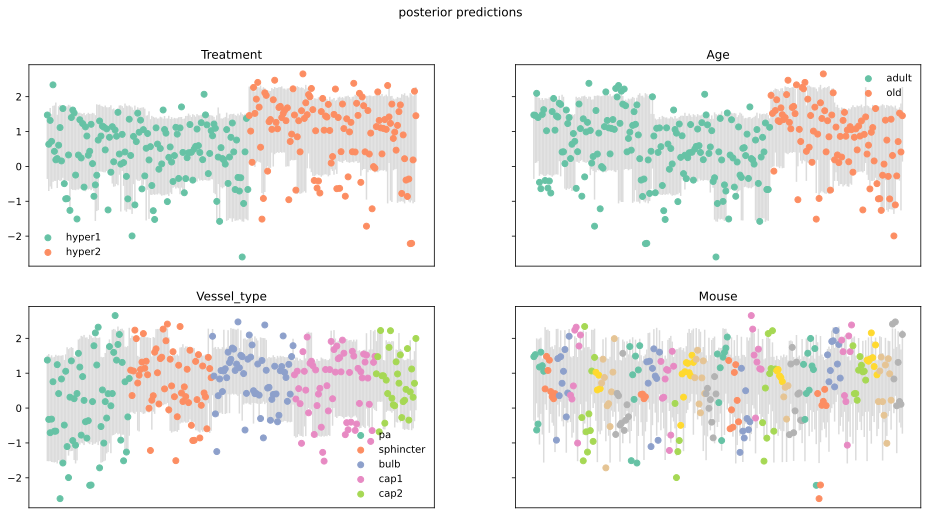
\includegraphics{../plots/hypertension-posterior-predictive.png}}

\end{figure}%

\section{Details of the density
analysis}\label{details-of-the-density-analysis}

The density dataset consisted of 144 measurements from five adult and
four old mice.

\subsection{Dependent variable}\label{dependent-variable-4}

The dependent variable in this case was vessel density, measured as in
length of vessel per unit of volume. These measurements are shown in
figure Figure~\ref{fig-density-measurements} on both natural and
logarithmic scales.

\begin{figure}

\centering{

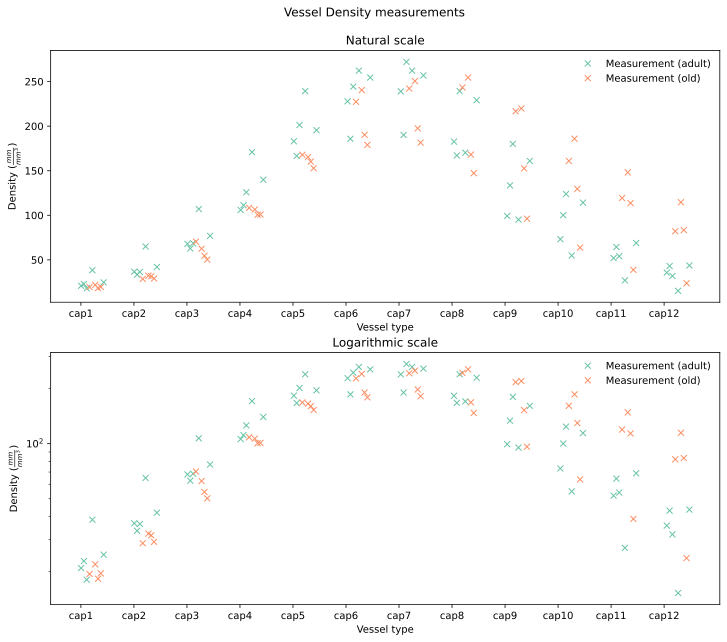
\includegraphics{../plots/density-measurements.png}

}

\caption{\label{fig-density-measurements}Vessel density measurements}

\end{figure}%

We noticed several interesting patterns in this data.

First, there is a clear trend for vessel density to increase with vessel
order until the cap6 vessel type and then to decrease, with adjacent
vessel types tending to have similar densities.

Second, the vessel types \texttt{pa} and \texttt{av} somewhat buck this
trend, with a similar upward deviation in both cases. These vessel
types---i.e.~penetrating arterioles and ascending venules---have the
common characterstic of being vertically oriented.

Finally, we noticed that the measurements are somewhat more dispersed
for higher-order capillaries, especially on log scale.

\subsection{Statistical model}\label{statistical-model-1}

We modelled the measurement process using a linear model on logarithmic
scale. In this model, given measurement \(y\), linear predictor
\(\hat{y}\) and measurement error parameter \(\sigma\), the measurement
probability density is given by this equation:

\begin{equation}
  p(y\mid\hat{y}, \sigma) = Normal(\ln{y}\mid hat{y}, \sigma) \label{eq:measurement-model-density}
\end{equation}

We modelled the linear predictor \(\hat{y}\) as depending on an
age-specific mean \(\mu\), an age and vessel type specific parameter
\(\alpha^{age,vessel type}\) and a scalar \(\alpha^{vert}\):

\begin{align}
  \hat{y} &= \mu_a \label{eq:density-measurement-model} \\
          &+ \alpha^{age:vesseltype}_{av} \nonumber \\ 
          &+ vert(v) \cdot \alpha^{vert} \nonumber
\end{align}

where \(vert(v)\) is an indicator function with value 1 if v represents
a vertical vessel and zero otherwise.

In order to capture the observed smoothness between adjacent vessel
types, we used Gaussian random walk priors for the
\(\alpha^{age:vesseltype}\) parameters for adult mice, and on the
differences at each vessel type between adult and old mice:

\begin{align}
  \alpha^{age:vesseltype}_{1v} &\sim N(\alpha^{age:vesseltype}_{1v-1}, \lambda_1)\label{eq:smooth} \\
  \delta_v &= \alpha^{age:vesseltype}_{2v} - \alpha^{age:vesseltype}_{1v} \nonumber \\
         &\sim N(\delta_{v-1}, \lambda_2) \nonumber
\end{align}

This approach to smoothing parameters corresponding to ordered
categories is essentially the same as that used in Gao et al. (2019) to
model age effects on voting behaviour. As explained in that paper, the
random walk priors allow for information sharing between categories,
without the need for detailed assumptions about the functional form of
the overall relationship.

The other priors in our model were as follows (units are on standardised
logarithmic scale):

\begin{align}
  \alpha^{vert} &\sim N(0, 0.1) \label{eq:density-other-priors} \\
  \mu &\sim N(0, 1) \nonumber \\
  \lambda_1 &\sim N(0, 0.3) \nonumber \\
  \lambda_2 &\sim N(0, 0.1) \nonumber \\
  \sigma &\sim N(0, 1) \nonumber \\
\end{align}

\subsection{Results}\label{results-4}

Figure~\ref{fig-density-ppc} shows the overall fit of our model to the
observed data. We judged that the overall fit to the observed
measurements was adequate and did not attempt model evaluation using
estimated leave-one-out density as given the highly correlated data it
would be difficult to perform the necessary estimates with acceptable
accuracy.

The one aspect of the data that our model does not adequately capture is
the increased dispersion in the measurements of high order capillaries.
We expect that this could be accounted for by adding a distributional
component to our model, but we judged that this would be unlikely to
dramatically change our results.

\begin{figure}

\centering{

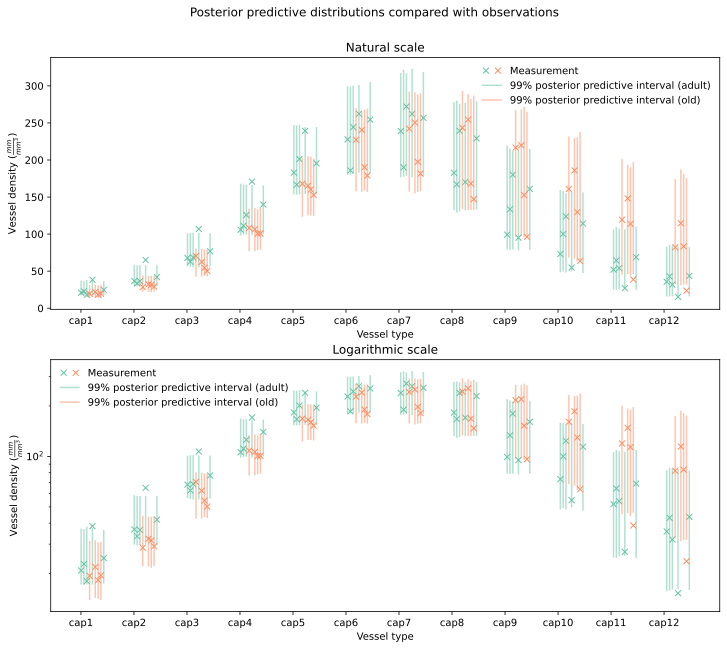
\includegraphics{../plots/density-ppc.png}

}

\caption{\label{fig-density-ppc}Posterior predictive check for our final
vessel density model, shown on natural and logarithmic scale.}

\end{figure}%

Figure~\ref{fig-density-effects-detail} shows posterior 94\% credible
intervals for the quantity
\((\mu_2 + \alpha^{age:vessel type}_2) - (\mu_2 + \alpha^{age:vessel
type}_2)\) for each vessel type; in other words, the overall difference,
on standardised log scale, in densities between old and adult mice for
each vessel type.

\begin{figure}

\centering{

\includegraphics{../plots/density-effects.png}

}

\caption{\label{fig-density-effects-detail}Main result of our density
analysis: old and adult mice have different vessel density patterns.}

\end{figure}%

There is a clear trend, with three low order capillary types separated
from zero on the left and five high order types separated on the right.

Finally, Figure~\ref{fig-density-mu} shows that, according to our model,
there is no particular effect of age on overall vessel density.

\begin{figure}

\centering{

\includegraphics{../plots/density-mu.png}

}

\caption{\label{fig-density-mu}Histogram of posterior samples for
overall age effects on density (old minus adult). The probability mass
does not concentrate away from zero, indicating no clear overall age
effect.}

\end{figure}%

\phantomsection\label{refs}
\begin{CSLReferences}{1}{0}
\bibitem[\citeproctext]{ref-betancourtDiagnosingBiasedInference2017}
Betancourt, Michael. 2017. {``Diagnosing {Biased Inference} with
{Divergences}.''} \emph{Betanalpha.github.io}.
\url{https://github.com/betanalpha/knitr_case_studies/tree/master/divergences_and_bias}.

\bibitem[\citeproctext]{ref-carpenterStanProbabilisticProgramming2017}
Carpenter, Bob, Andrew Gelman, Matthew D. Hoffman, Daniel Lee, Ben
Goodrich, Michael Betancourt, Marcus Brubaker, Jiqiang Guo, Peter Li,
and Allen Riddell. 2017. {``Stan: {A Probabilistic Programming
Language}.''} \emph{Journal of Statistical Software} 76 (1): 1--32.
\url{https://doi.org/10.18637/jss.v076.i01}.

\bibitem[\citeproctext]{ref-gaoImprovingMultilevelRegression2019}
Gao, Yuxiang, Lauren Kennedy, Daniel Simpson, and Andrew Gelman. 2019.
{``Improving Multilevel Regression and Poststratification with
Structured Priors.''} \emph{arXiv:1908.06716 {[}Stat{]}}, September.
\url{http://arxiv.org/abs/1908.06716}.

\bibitem[\citeproctext]{ref-gelmanBayesianWorkflow2020}
Gelman, Andrew, Aki Vehtari, Daniel Simpson, Charles C. Margossian, Bob
Carpenter, Yuling Yao, Lauren Kennedy, Jonah Gabry, Paul-Christian
Bürkner, and Martin Modrák. 2020. {``Bayesian Workflow.''}
\emph{arXiv:2011.01808 {[}Stat{]}}, November.
\url{https://arxiv.org/abs/2011.01808}.

\bibitem[\citeproctext]{ref-bibat}
Groves, Teddy. 2023. {``Bibat: Batteries-Included Bayesian Analysis
Template.''} \url{https://doi.org/10.5281/zenodo.7775328}.

\bibitem[\citeproctext]{ref-juarezModelBasedClusteringNonGaussian2010}
Juárez, Miguel A., and Mark F. J. Steel. 2010. {``Model-{Based
Clustering} of {Non-Gaussian Panel Data Based} on {Skew-t
Distributions}.''} \emph{Journal of Business \& Economic Statistics} 28
(1): 52--66. \url{https://doi.org/10.1198/jbes.2009.07145}.

\bibitem[\citeproctext]{ref-kumarArviZUnifiedLibrary2019}
Kumar, Ravin, Colin Carroll, Ari Hartikainen, and Osvaldo Martin. 2019.
{``{ArviZ} a Unified Library for Exploratory Analysis of {Bayesian}
Models in {Python}.''} \emph{Journal of Open Source Software} 4 (33):
1143. \url{https://doi.org/10.21105/joss.01143}.

\bibitem[\citeproctext]{ref-niels_bantilan-proc-scipy-2020}
Niels Bantilan. 2020. {``Pandera: {Statistical Data Validation} of
{Pandas Dataframes}.''} In \emph{Proceedings of the 19th {Python} in
{Science Conference}}, edited by Meghann Agarwal, Chris Calloway, Dillon
Niederhut, and David Shupe, 116--24.
\url{https://doi.org/10.25080/Majora-342d178e-010}.

\bibitem[\citeproctext]{ref-piironenSparsityInformationRegularization2017}
Piironen, Juho, and Aki Vehtari. 2017. {``Sparsity Information and
Regularization in the Horseshoe and Other Shrinkage Priors.''}
\emph{Electronic Journal of Statistics} 11 (2).
\url{https://doi.org/10.1214/17-EJS1337SI}.

\bibitem[\citeproctext]{ref-pydanticdevelopersPydantic2022}
Pydantic developers. 2022. {``Pydantic.''}
\url{https://pypi.org/project/pydantic/}.

\bibitem[\citeproctext]{ref-standevelopmentteamCmdStanPy2022}
Stan Development Team. 2022. {``{CmdStanPy}.''}
\url{https://github.com/stan-dev/cmdstanpy}.

\bibitem[\citeproctext]{ref-tornqvistHowShouldRelative1985}
Tornqvist, Leo, Pentti Vartia, and Yrjo O. Vartia. 1985. {``How {Should
Relative Changes Be Measured}?''} \emph{The American Statistician} 39
(1): 43--46. \url{https://doi.org/10.2307/2683905}.

\bibitem[\citeproctext]{ref-vehtariPracticalBayesianModel2017}
Vehtari, Aki, Andrew Gelman, and Jonah Gabry. 2017. {``Practical
{Bayesian} Model Evaluation Using Leave-One-Out Cross-Validation and
{WAIC}.''} \emph{Statistics and Computing} 27 (5): 1413--32.
\url{https://doi.org/10.1007/s11222-016-9696-4}.

\bibitem[\citeproctext]{ref-vehtariRankNormalizationFoldingLocalization2021}
Vehtari, Aki, Andrew Gelman, Daniel Simpson, Bob Carpenter, and
Paul-Christian Bürkner. 2021. {``Rank-{Normalization}, {Folding}, and
{Localization}: {An Improved R\^{}} for {Assessing Convergence} of
{MCMC} (with {Discussion}).''} \emph{Bayesian Analysis} 16 (2):
667--718. \url{https://doi.org/10.1214/20-BA1221}.

\end{CSLReferences}



\end{document}
